%! TEX root = report1_week4.tex
\documentclass[conference]{IEEEtran}

% --- Essential Packages ---
\usepackage[utf8]{inputenc}
\usepackage[T1]{fontenc}
\usepackage{newtxtext}
\usepackage{hyperref}
\usepackage{amsmath,amssymb}
\usepackage{graphicx}
\usepackage{booktabs}
\usepackage{listings}
\usepackage{xcolor}
\usepackage{float}



% --- Hyperref Setup ---
\hypersetup{
    colorlinks=true,
    linkcolor=black,        % Internal links (Table of Contents, references) stay black
    filecolor=magenta,      
    urlcolor=blue,          % Web URLs
    citecolor=black         % Citations stay black
}

% --- Code Listing Setup with Syntax Colors ---
\definecolor{codegreen}{rgb}{0.15,0.55,0.15}    % comments
\definecolor{codeblue}{rgb}{0.13,0.13,0.85}     % keywords (blue)
\definecolor{codefunc}{rgb}{0.50,0.25,0.0}      % functions / methods (warm amber / brown)
\definecolor{codepurple}{rgb}{0.55,0.0,0.55}    % strings
\definecolor{codegray}{rgb}{0.45,0.45,0.45}     % line numbers
\definecolor{codebg}{rgb}{0.97,0.97,0.98}       % light background
\definecolor{codeframe}{rgb}{0.85,0.85,0.85}    % border frame

\lstset{
    backgroundcolor=\color{codebg},
    commentstyle=\color{codegreen}\itshape,
    keywordstyle=\color{codeblue}\bfseries,
    keywordstyle=[2]\color{codefunc}\textbf,
    morekeywords=[2]{run, main, start, execute, shutdown, awaitTermination, getId, currentThread, newFixedThreadPool, println, print},
    numberstyle=\tiny\color{codegray},
    stringstyle=\color{codepurple},
    basicstyle=\ttfamily\scriptsize,
    breakatwhitespace=false,
    breaklines=true,
    captionpos=b,
    keepspaces=true,
    numbers=left,
    numbersep=4pt,
    showspaces=false,
    showstringspaces=false,
    showtabs=false,
    tabsize=2,
    frame=single,
    rulecolor=\color{codeframe}
}

% --- Document Information ---
\title{\textbf{COS40003: Concurrent Programming}\\
\Large Report 1: Learning Summary (Weeks 1--4)}

\author{\IEEEauthorblockN{Dang Duc Minh}
\IEEEauthorblockA{Student ID: 105559691}}

\pagestyle{plain}

\begin{document}

\maketitle
\thispagestyle{plain}

% ==============================================================================
% SECTION: WEEK 1 - INTRODUCTION TO CONCURRENT PROGRAMMING
% ==============================================================================
\section{Week 1 - Introduction}

\noindent The summary below for Week 1 covers \textbf{Part I} of \textbf{Lab 1}.

\subsection{Concurrent Computing}
% Perspective (observer's view), time-sharing, concurrency control
\textbf{Concurrent computing} is a fundamental computing paradigm that means multiple computational 
tasks are being executed on a same time period, but not necessarily 
simultaneously. Instead of processing tasks sequentially, the OS (operating system) will manages 
several execution flows at once to maximize resource utilization.

\hspace{5pt}

\noindent Concurrent computing relies heavily on \textbf{time-sharing}. The OS divides 
the CPU into small execution flows and rapidly switches between active processes. This approach
fundamentally maximizes system effciency by allowing processes that are ready to be executed to be
processed continously.

\hspace{5pt}

\noindent Coordinating concurrent tasks requires addresing two fundamental challanges:
 

\begin{enumerate}
    \item \textbf{Scheduling:} Determining which process executes next to ensure fairness and response time.
    \item \textbf{Concurrency Control:} Managing shared resources to prevent \textbf{race conditions} (inconsistent data or state caused by timing issues) and \textbf{deadlocks} (processes that wait indefinitely where two or more threads or processes wait indefinitely for each other, which prevents any of them from making progress).
\end{enumerate}

\noindent A common example of concurrent computing is a web browser (e.g., Chrome, Safari)
is opening multiple tabs at one, where each tab are doing seperate tasks such as playing a video, downloading a file,
or fetching live chat messages.

\hspace{5pt}

\noindent According to Rob Pike, co-creator of the Go programming language: 
\textbf{``concurrency is about dealing with lots of things at once, while parallelism is about doing lots of things at once''}~\cite{pike2012}.



\subsection{Parallel Computing}
% Perspective (system's view), hardware parallelism, subtask decomposition
\textbf{Parallel computing} is a computing architecture in which multiple calculations or execution flows
are carried out at the exact same time. Concurrent computing often creates an illusion of 
simultaneous progress on a single CPU from the user's perspective. Parallelism, on the other hand, represents multiple executions at the exact same time, as illustrated in Figure~\ref{fig:concurrent_vs_parallel}.

\begin{figure}[htbp]
    \centering
    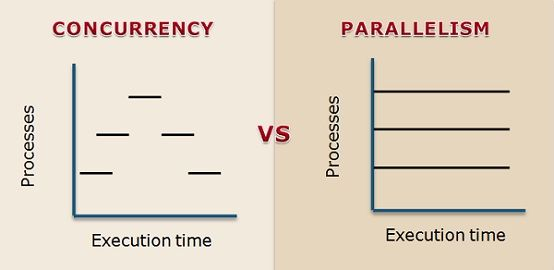
\includegraphics[width=0.7\columnwidth]{report1_images/parallel1.jpg}
    \caption{Concurrent execution vs. Parallel execution~\cite{techdifferences_concurrency_parallelism}.}
    \label{fig:concurrent_vs_parallel}
\end{figure}

\hspace{5pt}

\noindent In parallel computing, a large computational workload is broken down into smaller, independent subtasks that can be executed concurrently.
Each subtasks are executed simultaneously on seperate processors, and once they are finished, the individual sub-results are merged to produce the final
output. In a typical parallel computing architectures, processors communicate directly through \textbf{shared memory} to ensure
low-latency data exchange across processes.

\hspace{5pt}

\noindent A real-world example of parallel computing is a \textbf{Graphics Processing Unit (GPU)}, which 
comprises thousands of smaller arithmetic cores for executing identical operations such as rendering graphics or computing matrix multiplications
using the \textbf{Single Instruction, Multiple Data (SIMD) architecture} (shown in Figure~\ref{fig:simd}).

\begin{figure}[htbp]
    \centering
    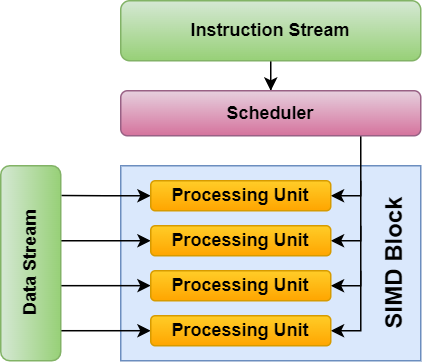
\includegraphics[width=0.6\columnwidth]{report1_images/parallel2.png}
    \caption{SIMD Architecture~\cite{rastergrid_simd_gpu}.}
    \label{fig:simd}
\end{figure}



\subsection{Distributed Computing}
% Autonomous nodes, private memory, message passing
Distributed computing consists of multiple autonomous computing entities that are connected through a shared network to solve complex computational problems.
A fundamental architectural distinction between parallel computing and distributed computing lies in memory organization. 
In parallel computing, processors shares a common memory space to exchange information directly. But for distributed computing, each individual computer cannot access each other's memory directly and must exchange information through \textbf{message passing} (communication protocols or middleware)~\cite{gfg_distributed_system}    (shown in Figure~\ref{fig:distributed_sys}).

\begin{figure}[htbp]
    \centering
    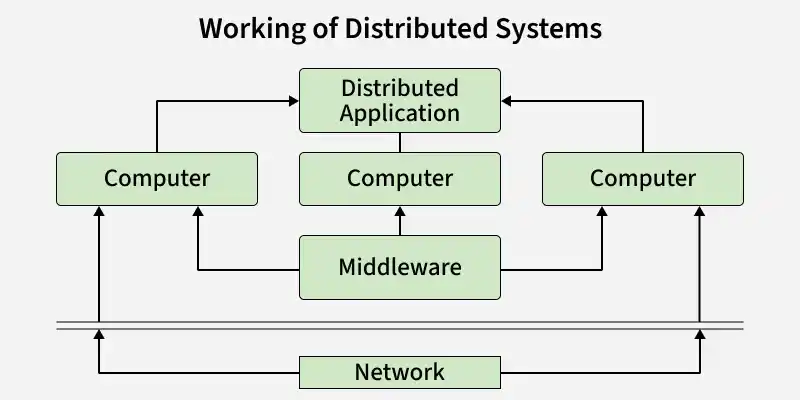
\includegraphics[width=0.7\columnwidth]{report1_images/distributed1.png}
    \caption{Architecture of a Distributed System~\cite{gfg_distributed_system}.}
    \label{fig:distributed_sys}
\end{figure}

\hspace{5pt}

\noindent Distributed computing architectures are commonly classified into two primary paradigms:

\begin{enumerate}
    \item \textbf{Cluster computing:} Composed of \textbf{homogeneous} machines, which feature similar hardware configurations and identical OSs, that are \textbf{co-located} within a single area. This architecture is designed for high availability and high-performance computing.
    \item \textbf{Grid computing:}  Comprised of \textbf{heterogeneous} computing entities that are \textbf{geographically dispersed} across different physical locations. Grid computing represents the conceptual predecessor to modern cloud infrastructure.
\end{enumerate}

\noindent A real-world example that implements both cluster and grid computing is the \textbf{Worldwide LHC Computing Grid (WLCG)}~\cite{cern_wlcg}. Local server
clusters are deployed for high-performance batch processing, and these clusters are linked globally into a centralized grid to analyze high volumes of data.

\subsection{Cloud Computing}
% Service abstraction (IaaS, PaaS, SaaS), distributed backend infrastructure

\textbf{Cloud Computing} is one of the most demanded computational infrastruture in modern computing, delivering services such as servers, storage, databases, and networking over the Internet. 

\hspace{5pt}

\noindent The fundamental goal of cloud computing is abstraction, which hides the underlying physical hardware and maintenance complexity from users, allowing them to access on demand resources with seamless scalability and minimal configuration. Behind this abstraction, cloud computing relies extensively on
distributed systems since it coordinates massive networks of server clusters to ensure high availability and data redundancy across multiple regions.

\hspace{5pt}

\noindent Cloud services are organized into three primary architectural models:

\begin{enumerate}
    \item \textbf{Infrastructure as a Service (IaaS):} Provides virtualized computing infrastructure, including virtual machines, block storage, and virtual networks (e.g., AWS EC2, Microsoft Azure VMs)
    \item \textbf{Platform as a Service (PaaS):} Provides a managed execution environment and development framework where developers can build and run applications without configuring the underlying OS or runtime (e.g., Vercel, Firebase)
    \item \textbf{Software as a Service (SaaS):} Provides software applications that can be directly accessed via web browsers (e.g., Microsoft 365, Google Docs).
\end{enumerate}

\begin{figure}[H]
    \centering
    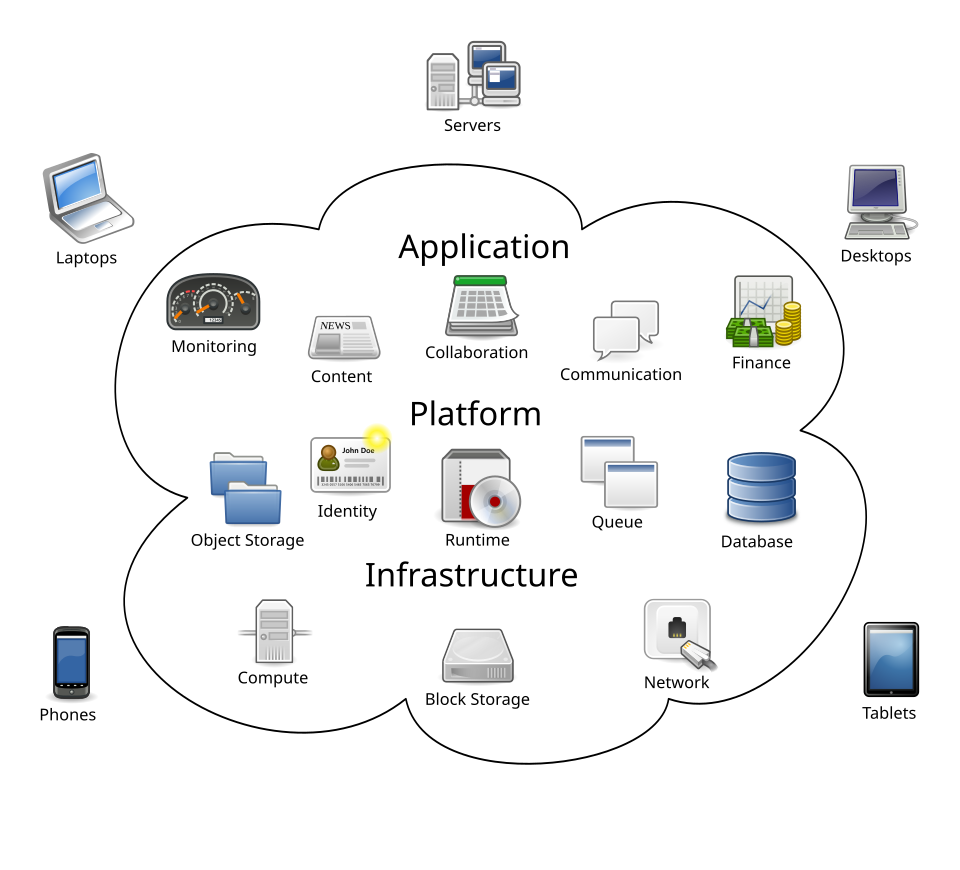
\includegraphics[width=0.65\columnwidth]{report1_images/cloud1.png}
    \caption{Cloud Computing Logical Architecture and Service Models~\cite{wiki_cloud_computing}.}
    \label{fig:cloud_computing}
\end{figure}

\subsection{Fog and Edge Computing}
% Proximity to data-generating devices, IoT applications, latency reduction

\textbf{Fog and Edge computing} designed to bring processing and data storage closer to data-generating sources, primarily Internet of Things (IoT) devices. These computing paradigms address the limitations of address critical limitations of cloud computing, such as transmission latency and bandwidth bottlenecks.

\begin{itemize}
    \item \textbf{Edge Computing:} Performs computation directly on local hardware devices such as microcontrollers, sensors, and local gateways.
    \item \textbf{Fog Computing:} Extends the cloud computing paradigm toward the physical local environment by introducing an intermediate layer that coordinates  compute resources between local devices (nodes) and the remote cloud.
\end{itemize}

\begin{figure}[H]
    \centering
    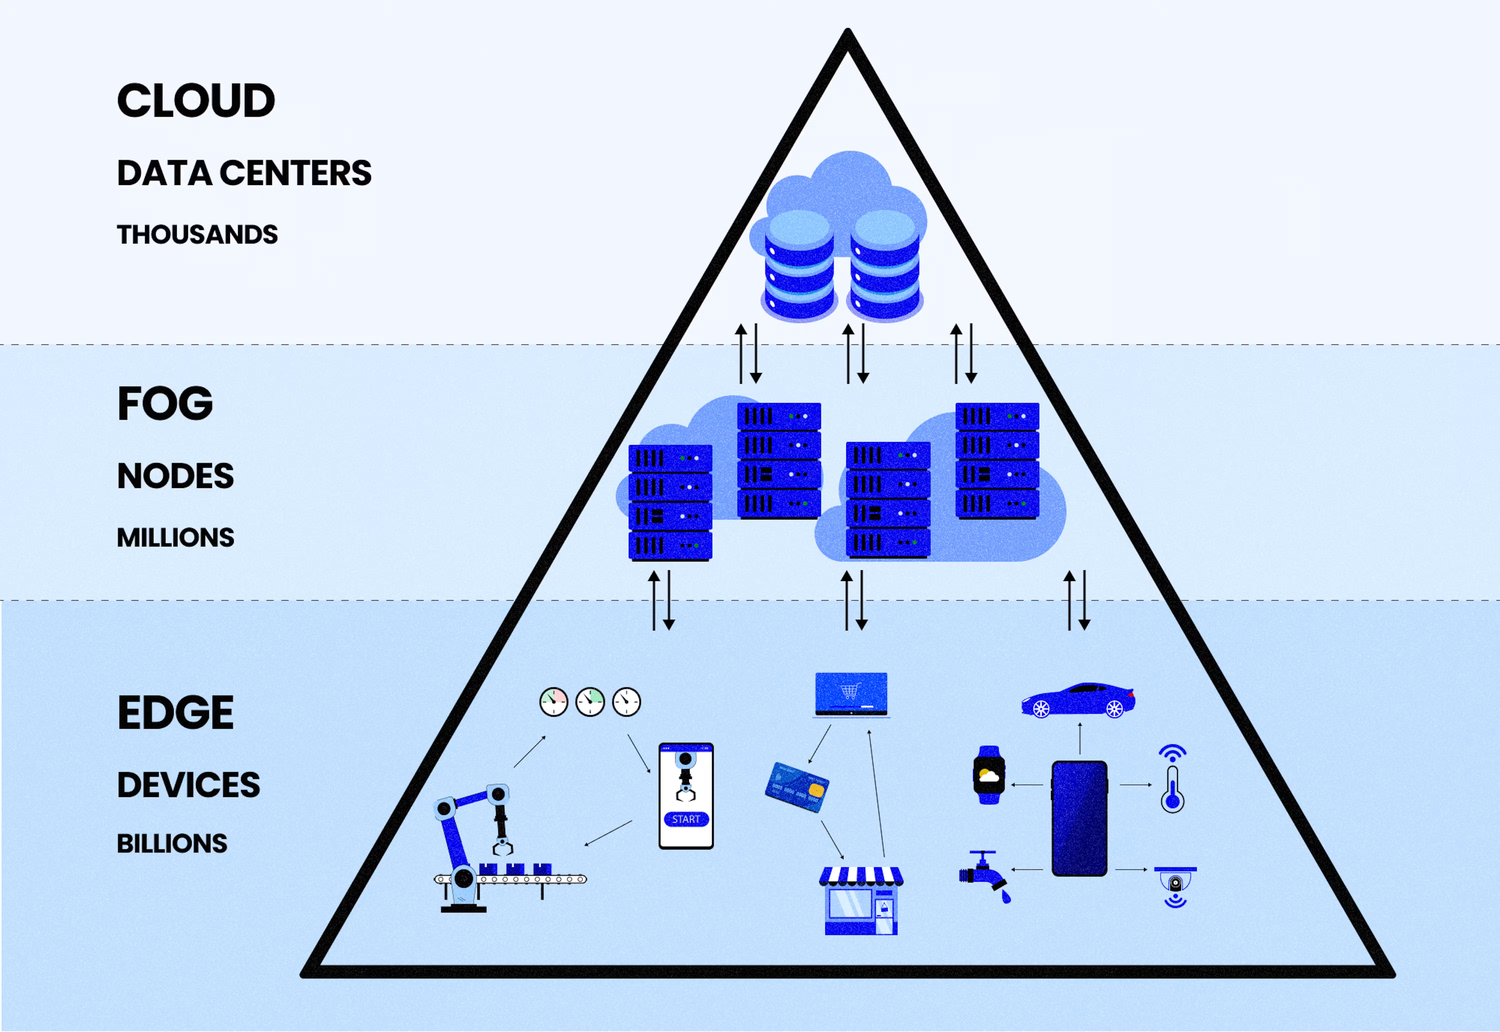
\includegraphics[width=0.6\columnwidth]{report1_images/fog_edge1.png}
    \caption{Edge Computing Architecture and Data Processing Flow~\cite{maddevs_edge_computing}.}
    \label{fig:fog_edge}
\end{figure}

\noindent A real-world implementation that utilizes both paradigms is smart traffic management in intelligent transportation systems~\cite{ieee_vehicular_fog}. Vehicle sensors process 
immediate collision data locally at the edge devices, while local base station units operate as an intermediate fog layer nodes to coordinate traffic
flow and signal timings in real time.

\subsection*{Lab 1 - Part II}

\begin{figure}[H]
    \centering
    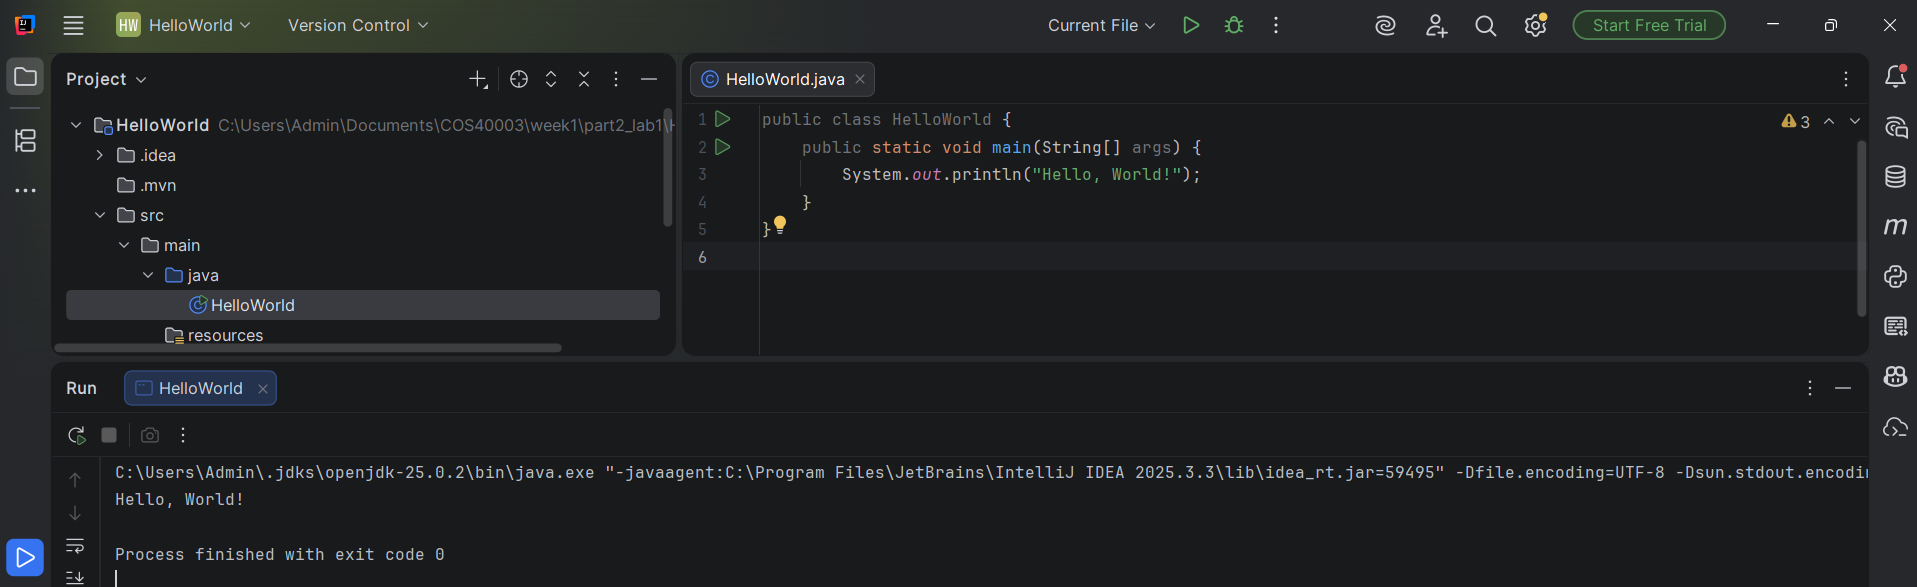
\includegraphics[width=\columnwidth]{report1_images/lab1_part2.png}
    \caption{The "Hello World!" Java application compiled and ran successfully.}
    \label{fig:lab1_part2}
\end{figure}



% ==============================================================================
% SECTION: WEEK 2 - PROCESS: CONCEPT AND API
% ==============================================================================
\section{Week 2 - Process: Concept and API}

\noindent The summary below for Week 2 covers \textbf{Part I} of \textbf{Lab 2}.

\subsection{Process Definition}

A process is essentially a program that being executed. When a process is running, the OS allocates
an address space in RAM (containing code, data, heap and stack) and the CPU read the instructions
and execute them on by one.

\hspace{5pt}

\noindent The differences between a process and a program lies in their execution state.
A program is stored as an executable binary on the disk, wheras a process is an active instance executing dynamically in memory.

\subsection{The Need for Processes}

Early computing executed single programs one at a time, which creates severe bottlenecks whenever a task had to wait for slow I/O operations, which forces the processor to idle. The 
abstraction of process was invented to solve this inefficiency, allows the OS to safely execute multiple programs concurrently with isolated memory.

\hspace{5pt}

\noindent The famous computer scientist Edsger W. Dijkstra has demonstrated the necessity of process through 
showing that breaking complex computing workloads into separated sequential execution units is essential to keep the CPU
continuously utilized while preventing tasks from overwriting shared data~\cite{dijkstra1968the}.

\subsection{Process Operations}

\subsubsection{Process Components}

A process comprises of four essential elements:
\begin{itemize}
    \item \textbf{Image of a program:} The compiled code, environment, and dependencies.
    \item \textbf{Memory (Address Space):} An isolated virtual address space allocated to each running process (shown in Figure~\ref{fig:process_address_space}). The program instructions data and static data remain fixed throughout execution, while two dynamic memory segments grow towards each other:
    \begin{figure}[H]
        \centering
        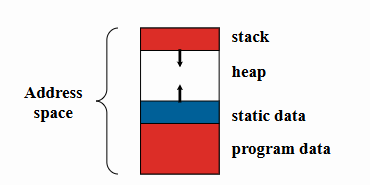
\includegraphics[width=0.65\columnwidth]{report1_images/process1.png}
        \caption{Process Address Space Structure~\cite{cos40003_lecture2}.}
        \label{fig:process_address_space}
    \end{figure}
    \begin{itemize}
        \item \textbf{Stack:} Managed automatically by the CPU in Last-In, First-Out (LIFO) order to store variables, function parameters, and return addresses. It grows downward toward lower memory addresses.
        \item \textbf{Heap:} Managed at runtime for for dynamic memory allocation. It grows upward toward higher memory addresses.
    \end{itemize}
    \item \textbf{CPU state:} Registers, Program Counter (PC), and Stack Pointer (SP).
    \item \textbf{OS state:} Metadatas such as opened files, temporal statistics, etc.
\end{itemize}

\subsubsection{Context Switch}

\textbf{Context switch} is a mechanism that alternates the CPU between different processes to enable multitasking. Because a single CPU core can execute only one process at a time, the OS rapidly switches active execution contexts between processes (represented as programs \texttt{Prog1} and \texttt{Prog2} in Figure~\ref{fig:context_switch}) across four phases:
\begin{enumerate}
    \item \textbf{Phase 1 (\texttt{Prog1} Running):} \texttt{Prog1} executes instructions on the CPU, while \texttt{Prog2} remains suspended.
    \item \textbf{Phase 2 (Save State):} The OS saves the CPU registers, PC, SP of \texttt{Prog1}, placing it into suspension.
    \item \textbf{Phase 3 (Restore State):} The OS restores the previously saved registers, PC, and SP belonging to \texttt{Prog2}.
    \item \textbf{Phase 4 (\texttt{Prog2} Running):} \texttt{Prog2} takes over the CPU and resumes execution, while \texttt{Prog1} waits in memory.
\end{enumerate}

\begin{figure}[H]
    \centering
    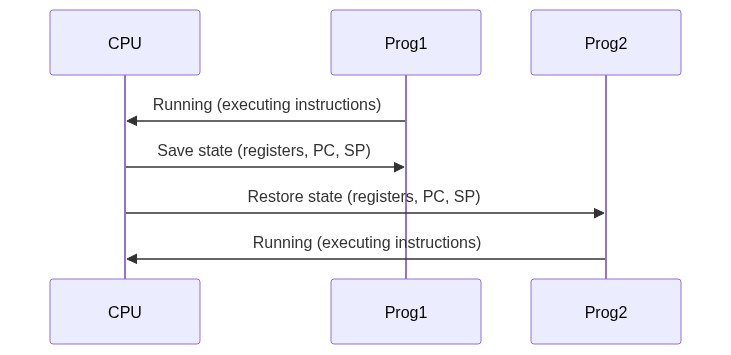
\includegraphics[width=0.8\columnwidth]{report1_images/process2.png}
    \caption{Process Context Switching Mechanism Between Two Processes.}
    \label{fig:context_switch}
\end{figure}

\subsubsection{The Process Abstraction}

The \textbf{process abstraction} is a conceptual bridge between shared physical hardware and private program execution processes:
\begin{itemize}
    \item \textbf{Physical View:} One physical CPU shared and context-switched among processes.
    \item \textbf{Logical View:} Each process operates as if it has its own dedicated CPU and memory.
    \item \textbf{Time-Sharing:} Processes rapidly take turns using the CPU, enabling multi-computational processes on a single core.
\end{itemize}

\subsubsection{Process States}

A process transitions through three primary execution states:
\begin{itemize}
    \item \textbf{Ready:} The process is loaded in memory and prepared to run.
    \item \textbf{Running:} The process currently holds the CPU and is actively executing instructions.
    \item \textbf{Blocked:} The process has released control of the CPU to wait for an event (such as I/O completion) and cannot execute until that event happens.
\end{itemize}

\noindent Transitions between these states occur as follows:
\begin{itemize}
    \item \textbf{Ready $\rightarrow$ Running:} The scheduler picks the process to run.
    \item \textbf{Running $\rightarrow$ Ready:} The scheduler suspends the process.
    \item \textbf{Running $\rightarrow$ Blocked:} The process waits for an event (e.g., I/O request).
    \item \textbf{Blocked $\rightarrow$ Ready:} The event occurs (e.g., I/O completes).
\end{itemize}

\subsection{Process APIs}

There are three fundamental process management APIs in Unix systems.

\begin{enumerate}
    \item \textbf{\texttt{fork()} - Creating a Process by Duplication:} 
    
    Creates an exact clone of the caller with its own memory space. It returns \texttt{0} to the child process and the child's Process ID (PID) to the parent, allowing both to branch into different execution paths.
    
    \item \textbf{\texttt{wait()} - Synchronizing with Child Termination:} 
    
    Pauses the calling parent until one of its child processes finishes execution. It returns the terminated child's PID and collects its exit status, preventing zombie processes (dead processes waiting for their parents).
    
    \item \textbf{\texttt{exec()} - Replacing Current Program Code:} 
    
    Replaces the process's current memory contents (code, data, heap, stack) with a new executable program from disk. The process retains its original PID but executes the new code.
\end{enumerate}

\newpage
\subsection*{Lab 2 - Part II}

\begin{figure}[H]
    \centering
    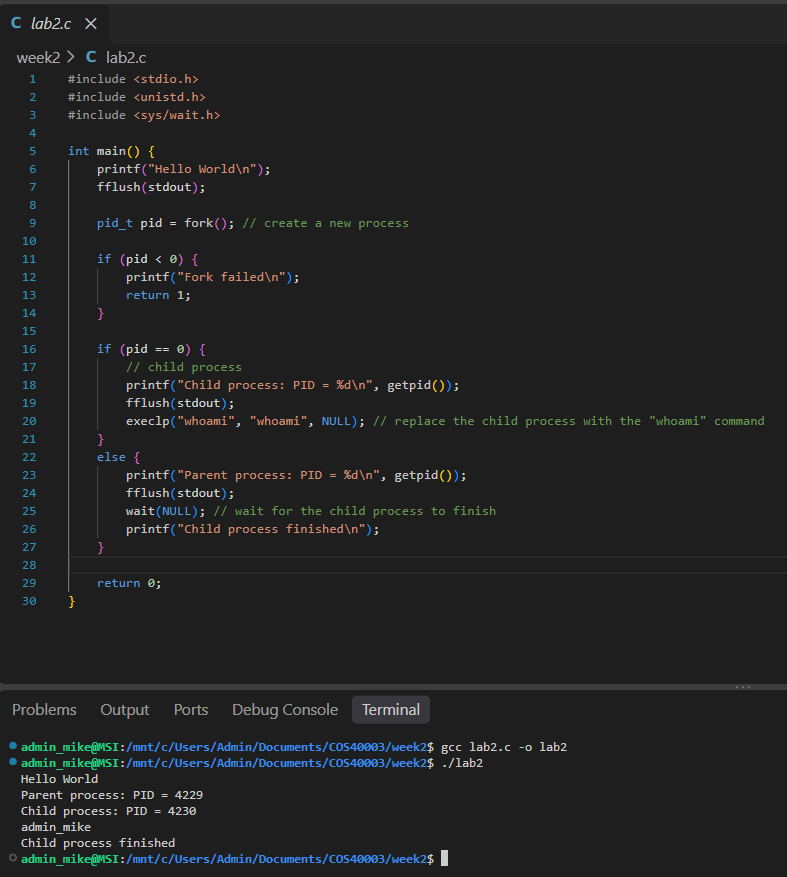
\includegraphics[width=0.65\columnwidth]{report1_images/lab2_part2.png}
    \caption{Example Hello World C Program using \texttt{fork()}, \texttt{wait()}, and \texttt{exec()} APIs.}
    \label{fig:lab2_part2}
\end{figure}

\section{Week 3 - Scheduling}

\noindent The summary below for Week 3 covers \textbf{Part I} of \textbf{Lab 3}.

\subsection{CPU Scheduling}

The OS must decide which process runs next on the CPU. This decision directly impacts system performance and the user experience. 

\hspace{5pt}

\noindent There are several \textbf{CPU Scheduling Criterias} that the OS can use:

\begin{itemize}
    \item \textbf{CPU Utilization:} The total time of the CPU being busy executing processes.
    \item \textbf{Turnaround Time:} The total time of a job submission to its termination.
    \item \textbf{Response Time:} The amount of time it takes to get the first response.
    \item \textbf{Missed Deadlines:} The number of jobs that fail to complete before their deadlines.
\end{itemize}

\noindent Beyond these performance criteria, there are several \textbf{CPU Scheduler Options} that define how scheduling policies are governed:

\begin{itemize}
    \item \textbf{Priorities:} Determines which process will be executed based on its priority level.
    \item \textbf{Preemptive vs. Non-preemptive:} 
    
    \begin{itemize}
    \item \textbf{Preemptive:} The OS can interrupt a running task at any time to take over.
    \item \textbf{Non-preemptive:} The OS will not interrupt a running task until it finishes its execution.
    
    \end{itemize}
\end{itemize}

\subsection {First-Come, First-Served (FIFO)}

The \textbf{First Come, First-Served algorithm} takes the first process that arrives and executes it until completion. Processes that comes next will wait in a queue until the CPU is avaliable (FIFO queue). 

\begin{figure}[htbp]
    \centering
    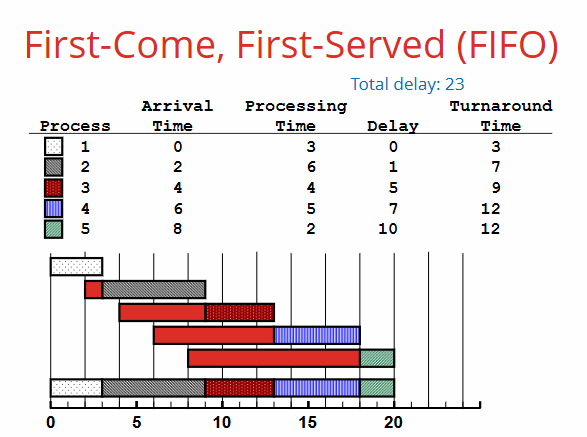
\includegraphics[width=0.7\columnwidth]{report1_images/FCFS1.png}
    \caption{FCFS Scheduling Example~\cite{cos40003_lecture3_1}.}
    \label{fig:fcfs}
\end{figure}

\noindent As shown in Figure~\ref{fig:fcfs}, five processes are scheduled non-preemptively based on their arrival times. Process 1 arrives at $t = 0$ and runs immediately, while subsequent processes must wait in the ready queue until the running task completes. Shorter processes that arrive later suffer significant waiting time such as Process 5, which requires only 2 units of processing time but experiences a delay of 10 units, which results in a high cumulative delay of 23 units. 

\subsection {Shortest Job First (non-preemptive)}

The \textbf{Shortest Job First (SJF) algorithm} selects the process with the shortest estimated execution time from the ready queue. This approach is non-preemptive, so that once a process starts executing, it will run to completion before the next process is selected.

\begin{figure}[htbp]
    \centering
    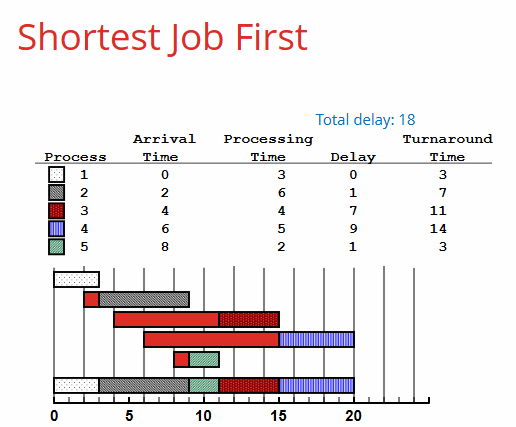
\includegraphics[width=0.7\columnwidth]{report1_images/SJF1.png}
    \caption{SJF Scheduling Example~\cite{cos40003_lecture3_1}.}
    \label{fig:sjf}
\end{figure}

\noindent As shown in Figure~\ref{fig:sjf}, after Process 1 and Process 2 complete at time unit 9, Process 5 is scheduled next because its required processing time is only 2 units, compared to 4 units for Process 3 and 5 units for Process 4. Prioritizing shorter jobs significantly decreases waiting time, bringing the total delay down to only 18 units.

\subsection {Shortest Job First (with preemption)}

The \textbf{Shortest Job First with preemption} also known as \textbf{Shortest Remaining Time (SRT)}. Whenever a new process arrives in the ready queue, the scheduler compares its total processing time against the remaining time of the currently running task. If the new process has a shorter remaining burst time, the OS will preempt the running process by moving it back to the ready queue, then immediately allocates the CPU to the new process. 

\begin{figure}[htbp]
    \centering
    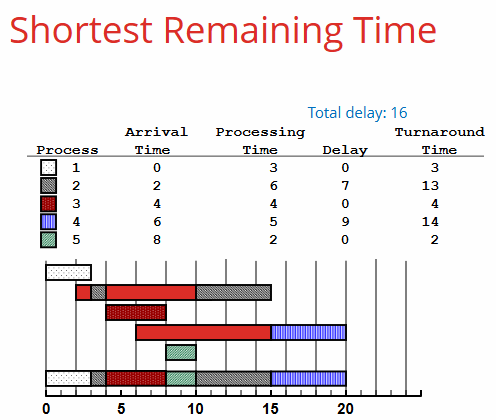
\includegraphics[width=0.7\columnwidth]{report1_images/SRT1.png}
    \caption{SRT Scheduling Example~\cite{cos40003_lecture3_1}.}
    \label{fig:srt}
\end{figure}

\noindent As shown in Figure~\ref{fig:srt}, at time unit 4, Process 3 preempts Process 2 because its required 4 units of processing time is shorter than the 5 units remaining for Process 2. Prioritizing shorter jobs immediately upon arrival allows Process 3 and Process 5 to finish with zero delay, reducing the total delay to 16 units. 

\newpage

\subsection {Round-Robin Scheduling}

The \textbf{Round-Robin (RR) Scheduling algorithm} limits the amount of time a process can run on the CPU to a fixed time slice (quantum). If the process does not finish within its allocated time, it is preempted for the next process in the queue. This approach ensures that all processes receive fair amount of CPU time.

\hspace{5pt}

\noindent The effectiveness of Round-Robin Scheduling depends on the the number of jobs and the size of the time quantum. Large number of jobs means that the time between scheduling of a single job increases, which inherently increases the waiting time. While larger time quantum means that the time between the scheduling of a single job also increases, which also increases the waiting time. However, smaller time quantum would leads to better response time but also increases overhead due to more frequent context switches.

\begin{figure}[htbp]
    \centering
    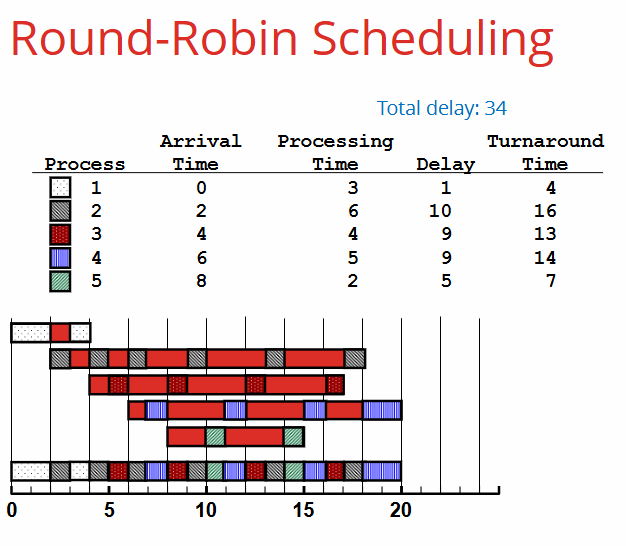
\includegraphics[width=0.7\columnwidth]{report1_images/RRS1.png}
    \caption{Round-Robin Scheduling Example~\cite{cos40003_lecture3_1}.}
    \label{fig:rrs}
\end{figure}

\noindent As shown in Figure~\ref{fig:rrs}, with a time quantum of 1 unit, the CPU continuously cycles through active jobs in the queue to grant each process immediate execution. Because execution is fragmented across different time slices, longer processes take much longer to reach final completion, which results in a high cumulative delay of 34 units.

\subsection {Lottery Scheduling}

The \textbf{Lottery Scheduling algorithm} is a type of proportional share scheduling in which the scheduler assigns a certain number of lottery tickets to each process. To select
the next process to run, the scheduler randomly generates a winning ticket number, and the process holding the matching ticket receives CPU execution time.

\hspace{5pt}

\noindent For example, if there are 100 total tickets and Process A holds 50 tickets, Process B
holds 15 tickets, and Process C holds 35 tickets, then Process A has a 50\% chance of being selected, Process B has a 15\% chance, and Process C has a 35\% chance. 

\subsection {Multi-Level Feedback Queue (MLFQ)}

The \textbf{Multi-Level Feedback Queue (MLFQ) algorithm} is designed to achieve two goals at once: 

\begin{enumerate}
    \item \textbf{Optimize Turnaround Time:} Algorithms like SJF or SRT are great for this, but we don't know the job lengths.
    \item \textbf{Minimize Response Time:} Algorithms like RR are great for this, but produce terrible turnaround time.
\end{enumerate}

\noindent MLFQ uses multiple queues with different priority levels. There are several rules that govern how processes are scheduled and moved between queues:

\vspace{0.3em}
\noindent \textbf{Rule 1:} If $\text{Priority}(A) > \text{Priority}(B)$, $A$ runs and $B$ doesn't. \\[0.3em]
\noindent \textbf{Rule 2:} If $\text{Priority}(A) = \text{Priority}(B)$, $A$ and $B$ run in RR. \\[0.3em]
\noindent \textbf{Rule 3:} When a job enters the system, it is placed at the highest-priority queue. \\[0.3em]
\noindent \textbf{Rule 4a:} If a job uses up an entire time slice while running, its priority is reduced. \\[0.3em]
\noindent \textbf{Rule 4b:} If a job gives up the CPU before the time slice is up, it stays at the same priority level.

\begin{figure}[htbp]
    \centering
    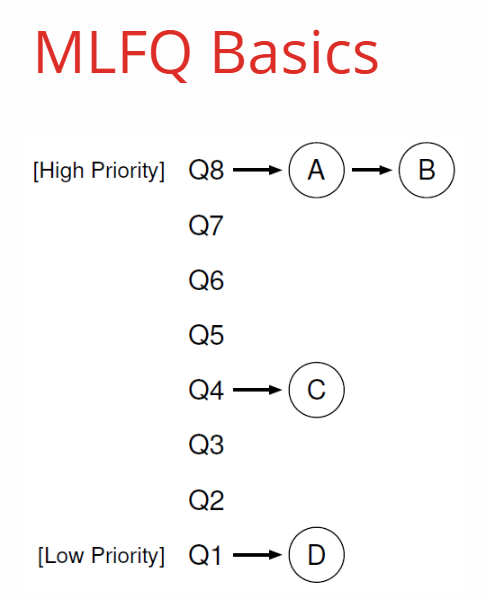
\includegraphics[width=0.65\columnwidth]{report1_images/MLFQ1.png}
    \caption{Multi-Level Feedback Queue Example~\cite{cos40003_lecture3_1}.}
    \label{fig:mlfq}
\end{figure}

\noindent As shown in Figure~\ref{fig:mlfq}, processes are distributed across priority tiers from Q8 to Q1. The scheduler selects jobs from the highest queue, executing Process A and Process B in RR at Q8 while Process C (at Q4) and Process D (at Q1) wait.

\subsection*{Lab 3 - Part II}

\noindent \textbf{What are the main tasks of the scheduler?} 
Allocating CPU time to jobs, measuring time slices, assigning job priorities, and preempting running tasks when necessary.

\hspace{5pt}

\vspace{0.3em}
\noindent \textbf{What is the difference between preemptive and non-preemptive scheduling?} 
Preemptive scheduling allows the operating system to actively interrupt and suspend running processes, while non-preemptive scheduling allows processes to run until they complete.

\hspace{5pt}


\vspace{0.3em}
\noindent \textbf{What is the advantage of a shorter scheduling quantum?} 
It reduces response time because there is a shorter delay time between execution turns.

\hspace{5pt}

\vspace{0.3em}
\noindent \textbf{What is the advantage of a longer scheduling quantum?} 
It results in fewer context switches, which reduces system overhead.

\hspace{5pt}

\vspace{0.3em}
\noindent \textbf{Why is feedback scheduling useful for interactive jobs?} 
Interactive tasks are usually much shorter and frequently start and stop. Because feedback scheduling assigns every new task the highest priority, interactive jobs are run at the highest priority.

\hspace{5pt}

\vspace{0.3em}
\noindent \textbf{Are these scheduling policies subject to starvation?} 

\begin{itemize}
    \item \textbf{Shortest Job First scheduling?} Yes, longer jobs can starve if shorter jobs continuously arrive.
    \item \textbf{Round Robin scheduling?} No, every job is guaranteed CPU time within a bounded time quantum cycle.
    \item \textbf{First Come First Served scheduling?} No, jobs are processed in strict arrival order, so every job will eventually execute.
    \item \textbf{Fixed Priority scheduling?} Yes, lower-priority jobs will starve if higher-priority jobs keep occupying the CPU.
    \item \textbf{Multi-level feedback scheduling?} No, because priority boost moves all jobs back to the highest-priority queue periodically.
\end{itemize}

\section{Week 4 - Thread}

\noindent The summary below for Week 4 covers \textbf{Part I} of \textbf{Lab 4}.

\subsection{The Need for Threads}

\noindent The invention of processes has enabled OS-level multitasking, but it is not enough for subtasks within a single application due to heavy context-switch costs, data redundancy, and expensive Inter-Process Communication (IPC). 
\noindent Therefore, thread was introduced to enable concurrent subtasks within a shared address space.

\hspace{5pt}

\noindent According to benchmark measurements published by the Lawrence Livermore National Laboratory, creating 50,000 processes required 8.1 seconds while creating the same amount of threads only took 0.9 seconds on an Intel Xeon CPU ~\cite{llnl_posix}.
This comparision demonstrated that thread creation requires lower operating system overhead than process creation.

\subsection{Thread Definition}

\noindent Threads are running subtasks of a process that execute instruction sequences concurrently within the same virtual address space. Threads have their own CPU context for independent control flow:

\begin{itemize}
    \item \textbf{Program Counter (PC):} Tracks the address of the next instruction to execute.
    \item \textbf{Stack Pointer (SP) \& Stack (memory):} Manages local variables, function calls, and return addresses.
    \item \textbf{Register States (CPU):} Holds temporary values and states for execution
\end{itemize}

\noindent Unlike a traditional process (single-threaded), which contains only a single stack for one execution flow, a multi-threaded process can execute multiple instruction streams simultaneously while sharing the same program code and heap memory.

\begin{figure}[H]
    \centering
    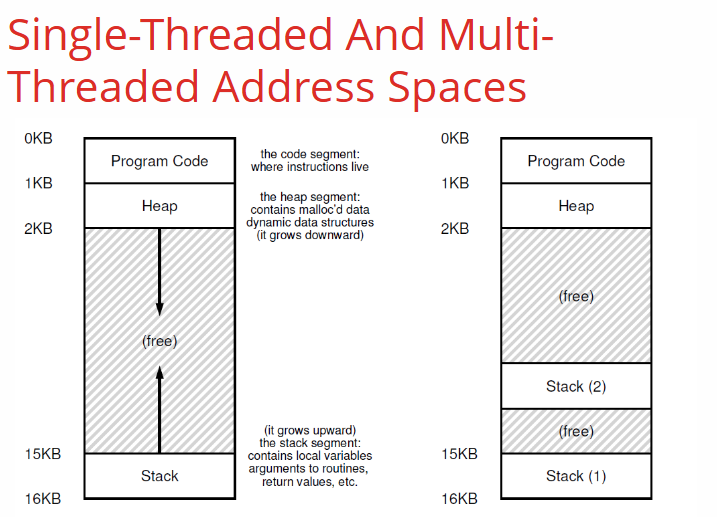
\includegraphics[width=0.7\columnwidth]{report1_images/thread1.png}
    \caption{Single-Threaded vs. Multi-Threaded Address Spaces ~\cite{cos40003_lecture4_1}.}
    \label{fig:single_vs_multi_threaded}
\end{figure}

\subsection*{Thread States:}
\begin{itemize}
    \item \textbf{Private Per-Thread State:} Elements that define the state of a particular flow of control in an executing program (PC, SP, Registers, Stack (local variables), Scheduling properties).
    \item \textbf{Shared State Among Threads (Process-Level):} The resources and memory shared by all threads residing in the same process (process identifiers (user ID, group ID, process ID), address space (program instructions, static data, heap and stack memory), and operating system resources (opened files, network sockets, and locks)).
\end{itemize}


\subsection{Thread Operations}

\noindent The program is split into multiple routines in order to execute in parallel. 
This execution results in either \textbf{true parallelism} (running simultaneously across multiple CPU cores) or \textbf{pseudo (interleaved) parallelism} (simulated on a single CPU core through rapid context-switching).

\subsubsection{Thread Strategies}

\begin{itemize}
    \item \textbf{Manager:} A single manager thread handles I/O, assigns work to worker threads.
    \item \textbf{Worker:} Worker threads can be created dynamically or allocated from a thread pool.
    \item \textbf{Pipeline:} Each thread handles a distinct stage of an assembly line, handing work to each other in a producer-consumer relationship
\end{itemize}

\begin{figure}[H]
    \centering
    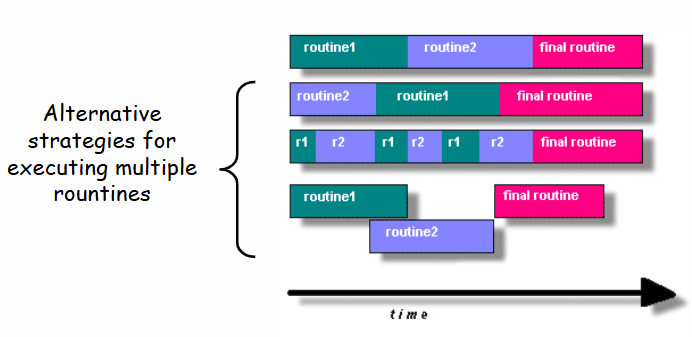
\includegraphics[width=0.7\columnwidth]{report1_images/thread2.png}
    \caption{Alternative Strategies for Executing Multiple Routines ~\cite{cos40003_lecture4_1}.}
    \label{fig:thread_execution_strategies}
\end{figure}

\subsubsection{Pthreads API}

\noindent \texttt{Pthreads} is a POSIX standard thread library. 
The first thread exists in \texttt{main()} and creates all subsequent threads.

\begin{table}[H]
    \centering
    \footnotesize
    \begin{tabular}{p{2.6cm}p{5.4cm}}
        \toprule
        \textbf{Function} & \textbf{Description} \\
        \midrule
        \texttt{pthread\_create()} & Creates a new thread executing the routine specified by \texttt{start\_routine(arg)} and returns its thread ID in \texttt{thread}. \\
        \addlinespace
        \texttt{pthread\_exit()} & Terminates the calling thread and passes its return \texttt{status} to any joining thread. \\
        \addlinespace
        \texttt{pthread\_join()} & Blocks the calling thread until the thread specified by \texttt{threadid} terminates, enabling synchronization between threads. \\
        \addlinespace
        \texttt{pthread\_yield()} & Allows the calling thread to give up the CPU and re-enter the OS's run queue. \\
        \bottomrule
    \end{tabular}
    \caption{Core \texttt{Pthreads} Management APIs.}
    \label{tab:pthreads_apis}
\end{table}

\begin{figure}[H]
    \centering
    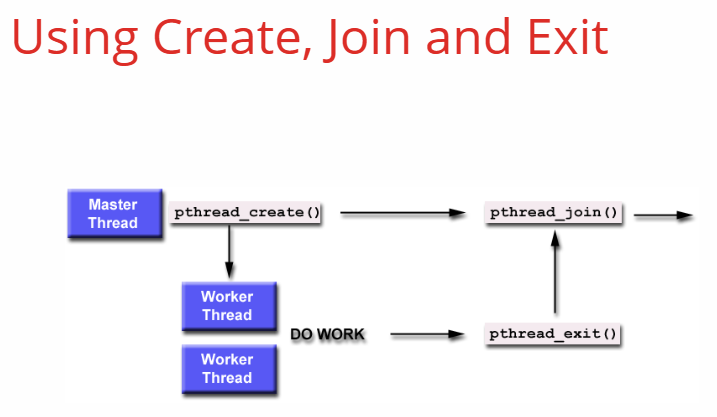
\includegraphics[width=0.7\columnwidth]{report1_images/thread3.png}
    \caption{Thread Lifecycle and Synchronization Workflow using \texttt{create()}, \texttt{join()}, and \texttt{exit()~\cite{cos40003_lecture4_1}}.}
    \label{fig:thread_create_join_exit}
\end{figure}





\subsection{Thread in Java}

\noindent Java provides built-in multithreading support via the \texttt{Thread} class and the \texttt{Runnable} interface:

\subsubsection*{\texttt{Thread} class}

\noindent The \texttt{Thread} class executes instructions from its \texttt{run()} method, which is implemented in a derived class. Calling \texttt{.start()} to get the thread ready to run, and the thread terminates when its \texttt{run()} method finishes.

\begin{lstlisting}[language=Java, caption={Creating a thread by extending the \texttt{Thread} class.}]
class MyThread extends Thread {
    @Override
    public void run() {
        System.out.println("Thread " + Thread.currentThread().getId() + " is running");
    }
}

public class Main {
    public static void main(String[] args) {
        Thread t = new MyThread();
        t.start(); // Call .start() to get the thread ready to run
    }
}
\end{lstlisting}

\newpage

\subsubsection*{\texttt{Runnable} interface}

\noindent Implementing the \texttt{Runnable} interface provides the \texttt{run()} method implementation, which is then then passed to a \texttt{Thread} object to execute.

\begin{lstlisting}[language=Java, caption={Creating a thread by implementing the \texttt{Runnable} interface.}]
class MyTask implements Runnable {
    @Override
    public void run() {
        System.out.println("Task running on Thread " + Thread.currentThread().getId());
    }
}

public class Main {
    public static void main(String[] args) {
        Thread t = new Thread(new MyTask());
        t.start();
    }
}
\end{lstlisting}

\hspace{5pt}

\noindent These are some core Java \texttt{Thread} methods:

\begin{table}[H]
    \centering
    \footnotesize
    \begin{tabular}{p{2.6cm}p{5.4cm}}
        \toprule
        \textbf{Method} & \textbf{Description} \\
        \midrule
        \texttt{.start()} & Begins a thread running by scheduling it to execute \texttt{run()} asynchronously. \\
        \addlinespace
        \texttt{wait() / notify()} & Used for inter-thread synchronization and conditional coordination. \\
        \addlinespace
        \texttt{.stop()} & Kills a specific thread (deprecated). \\
        \addlinespace
        \texttt{.suspend() / .resume()} & Suspends and resumes thread execution (deprecated). \\
        \addlinespace
        \texttt{.join()} & Waits for a specific thread to finish execution before continuing. \\
        \addlinespace
        \texttt{.setPriority()} & Sets thread priority from 1 to 10 (\texttt{MIN\_PRIORITY} to \texttt{MAX\_PRIORITY}); default is 5 (\texttt{NORM\_PRIORITY}). \\
        \bottomrule
    \end{tabular}
    \caption{Core Java \texttt{Thread} Methods.}
    \label{tab:java_thread_methods}
\end{table}

\subsubsection{Thread Safety in Java Libraries}

\noindent In the standard Java library, not all classes are thread-safe:

\begin{itemize}
    \item \textbf{Thread-Safe:}
    \begin{itemize}
        \item Most classes in \texttt{java.lang} (e.g., immutable types like \texttt{String}, \texttt{Integer}).
        \item \texttt{java.util.Random} (designed for safe concurrent number generation).
        \item \texttt{System.out} (safe concurrent output streams).
    \end{itemize}
    \item \textbf{NOT Thread-Safe:}
    \begin{itemize}
        \item Most standard collections in \texttt{java.util} (\texttt{ArrayList}, \texttt{HashMap}, \texttt{LinkedList}, \texttt{HashSet}). Multiple threads modifying an \texttt{ArrayList} simultaneously can corrupt its internal arrays.
        \item Java GUI frameworks (\texttt{javax.swing}, \texttt{java.awt}). Modifying GUI components from background threads may lead to invalid visual state.
    \end{itemize}
\end{itemize}

\subsubsection{Atomicity}

\noindent An operation is atomic if it executes as indivisible steps. 
In Java, integer increment (\texttt{count++}) is not atomic. It consists of three seperate operations:

\begin{itemize}
    \item[1.] Load data from variable \texttt{i}
    \item[2.] Increment data by 1
    \item[3.] Store data to variable \texttt{i}
\end{itemize}

\subsubsection{Thread Pools}

\noindent A program that creates a huge number of short-lived threads can be inefficient since threads are managed by the OS, which introduces significant memory overhead.
The cost can be reduced by using \textbf{thread pool} which pre-allocate a fixed number of worker threads and keep them alive to execute tasks repeatedly.

\hspace{5pt}

\noindent A notable example of thread pool is in client-server architecture such as web servers, particularly where a high volume of short-lived client requests arrive concurrently.
To avoid the overhead of creating a new thread for each connection, the server uses a fixed pool of worker threads to process incoming requests efficiently without exhausting system resources.

\hspace{5pt}

\noindent Thread pool works by maintaining a task queue with a fixed set of pre-allocated worker threads. 
When the queue is empty, worker threads sleep via \texttt{wait()}.
When a new task arrives, an idle worker thread will be notified to dequeue and execute it.
After that task is completed, the worker thread will return to the pool to execute subsequent tasks or wait for new tasks.

\hspace{5pt}

\subsubsection*{Thread Pools Java API}

\noindent In Java, thread pools are provided by the \texttt{java.util.concurrent} package, with \texttt{ThreadPoolExecutor} serving as the implementation of the \texttt{ExecutorService} interface. Its core methods include:

\begin{itemize}
    \item \texttt{execute()}: Creates a new thread inside the \texttt{ExecutorService} and returns immediately from each invocation.
    \item \texttt{shutdown()}: Initiates an orderly shutdown in which previously submitted tasks are executed, but no new tasks will be accepted.
    \item \texttt{awaitTermination()}: Waits for submitted tasks to finish. The program will not terminate until its last thread completes execution .
\end{itemize}

\begin{lstlisting}[language=Java, caption={Thread Pool implementation using \texttt{ExecutorService}.}]
import java.util.concurrent.ExecutorService;
import java.util.concurrent.Executors;
import java.util.concurrent.TimeUnit;

public class ThreadPoolExample {
    public static void main(String[] args) throws InterruptedException {
        // Create a fixed thread pool with 3 worker threads
        ExecutorService executor = Executors.newFixedThreadPool(3);

        // Submit tasks to the executor
        executor.execute(new Task());
        executor.execute(new Task());
        executor.execute(new Task());

        // Orderly shutdown and wait for tasks to finish
        executor.shutdown();
        executor.awaitTermination(1, TimeUnit.MINUTES);
    }
}
\end{lstlisting}

\newpage

\subsection*{Lab 4 - Part II}

\noindent \textbf{(1): Example 1}

\begin{figure}[H]
    \centering
    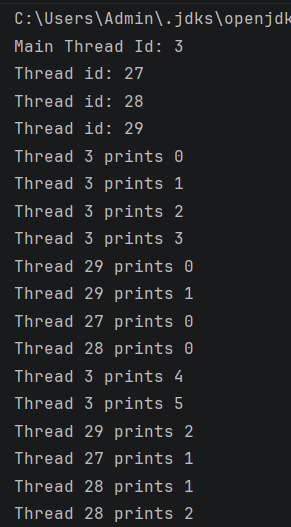
\includegraphics[width=0.3\columnwidth]{report1_images/lab4_part2_1.png}
    \caption{Console output from running \texttt{Thread1.java} (\texttt{example1}).}
    \label{fig:lab4_part2_1}
\end{figure}

\begin{figure}[H]
    \centering
    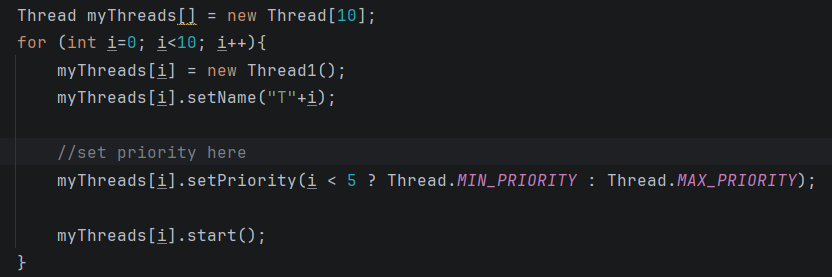
\includegraphics[width=0.8\columnwidth]{report1_images/lab4_part2_2.png}
    \caption{Setting thread priorities in \texttt{Thread1.java} (\texttt{example1b}).}
    \label{fig:lab4_part2_2}
\end{figure}

\noindent Thread priority is configured using \texttt{setPriority()} before invoking \texttt{start()}. It range from \texttt{Thread.MIN\_PRIORITY} (which is 1, the lowest scheduling preference) to \texttt{Thread.MAX\_PRIORITY} (which is 10, the highest scheduling preference) ~\cite{oracle_concurrency}. 

\begin{figure}[H]
    \centering
    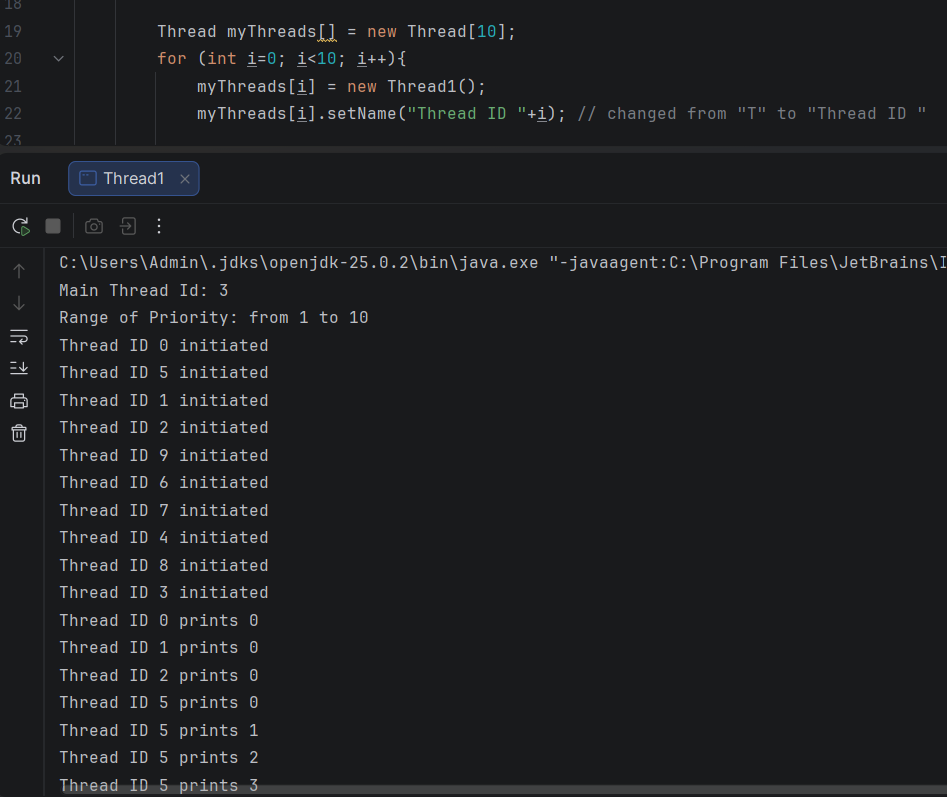
\includegraphics[width=0.7\columnwidth]{report1_images/lab4_part2_3.png}
    \caption{Changed the thread name using \texttt{setName()} in \texttt{Thread1.java} (\texttt{example1b}).}
    \label{fig:lab4_part2_3}
\end{figure}

\noindent A thread's name can be configured using the \texttt{setName()} method. 

\newpage

\noindent \textbf{(2): Example 2}

\begin{figure}[H]
    \centering
    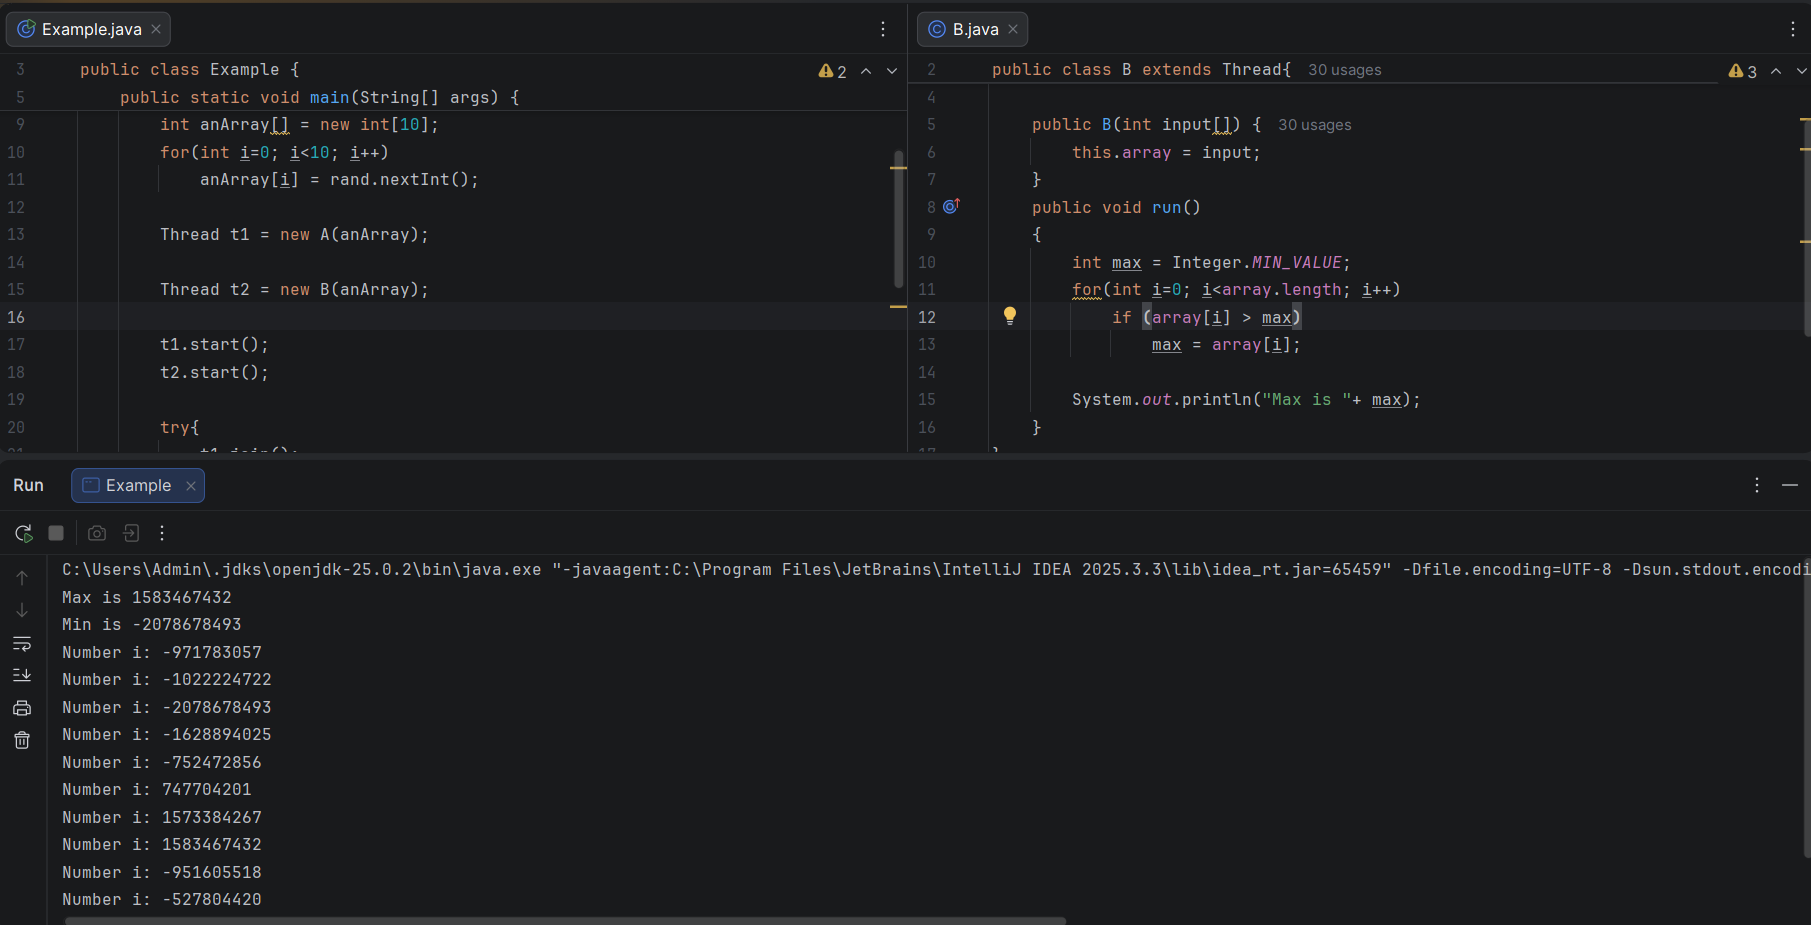
\includegraphics[width=0.9\columnwidth]{report1_images/lab4_part2_4.png}
    \caption{Implementation and execution of \texttt{example2b}.}
    \label{fig:lab4_part2_4}
\end{figure}

\noindent \textbf{(3): Example 3}

\begin{figure}[H]
    \centering
    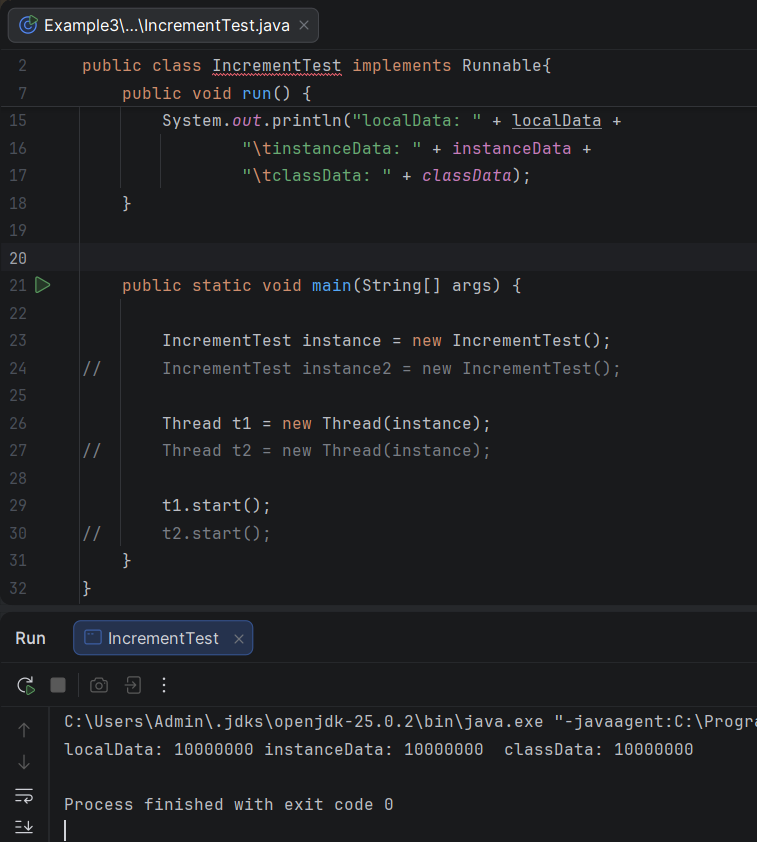
\includegraphics[width=0.6\columnwidth]{report1_images/lab4_part2_5.png}
    \caption{Execution of a single thread \texttt{t1} (\texttt{example3}).}
    \label{fig:lab4_part2_5}
\end{figure}
\begin{figure}[H]
    \centering
    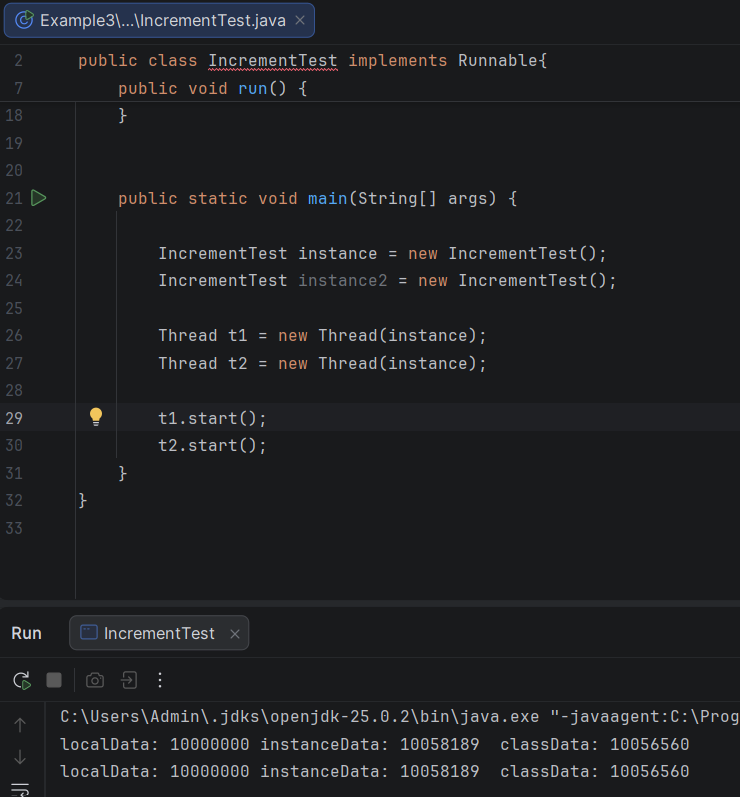
\includegraphics[width=0.6\columnwidth]{report1_images/lab4_part2_6.png}
    \caption{Concurrent execution of two threads \texttt{t1} and \texttt{t2} (\texttt{example3}).}
    \label{fig:lab4_part2_6}
\end{figure}
\begin{figure}[H]
    \centering
    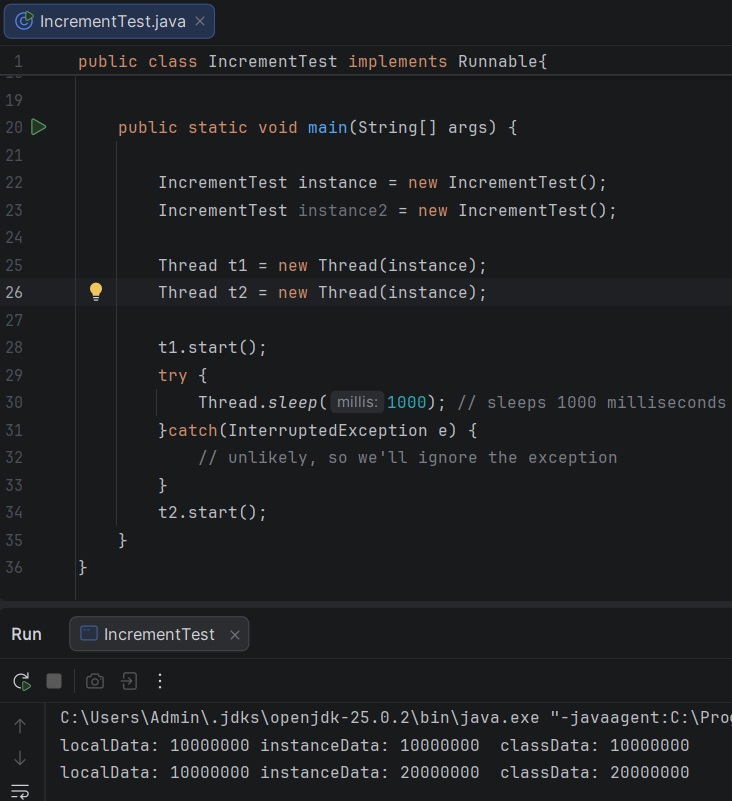
\includegraphics[width=0.6\columnwidth]{report1_images/lab4_part2_7.png}
    \caption{Concurrent execution of two threads \texttt{t1} and \texttt{t2} with \texttt{Thread.sleep(1000)} (\texttt{example3b}).}
    \label{fig:lab4_part2_7}
\end{figure}
\noindent As \texttt{Thread.sleep(1000)} pauses added to the main thread which allows \texttt{t1} to finish completely before \texttt{t2} starts. 
Two threads running sequentially will prevent race conditions, so both \texttt{instanceData} and \texttt{classData} correctly reach \texttt{20000000}.


% ==============================================================================
% REFERENCES
% ==============================================================================
\begin{thebibliography}{99}
\raggedright

\bibitem{pike2012}
R. Pike, ``Concurrency is not Parallelism,'' presented at \emph{Heroku Waza}, San Francisco, CA, USA, 2012. [Online]. Available: \url{https://go.dev/talks/2012/waza.slide#8}. 

\bibitem{techdifferences_concurrency_parallelism}
TechDifferences, ``Difference Between Concurrency and Parallelism,'' \emph{TechDifferences}, [Online]. Available: \url{https://techdifferences.com/difference-between-concurrency-and-parallelism.html}. 

\bibitem{rastergrid_simd_gpu}
D. Rákos, ``SIMD in the GPU world,'' \emph{RasterGrid Blog}, Feb. 2022. [Online]. Available: \url{https://www.rastergrid.com/blog/gpu-tech/2022/02/simd-in-the-gpu-world/}. 

\bibitem{gfg_distributed_system}
GeeksforGeeks, ``What is a Distributed System? Architecture and Components,'' \emph{GeeksforGeeks}, [Online]. Available: \url{https://www.geeksforgeeks.org/computer-networks/what-is-a-distributed-system/}. 

\bibitem{cern_wlcg}
CERN, ``The Worldwide LHC Computing Grid (WLCG),'' \emph{CERN}, [Online]. Available: \url{https://wlcg.web.cern.ch/}. 

\bibitem{wiki_cloud_computing}
Wikipedia, ``Cloud Computing,'' \emph{Wikimedia Commons}, [Online]. Available: \url{https://en.wikipedia.org/wiki/Cloud_computing#/media/File:Cloud_computing.svg}. [Accessed: Sep. 27, 2026].

\bibitem{ieee_vehicular_fog}
Z. Ning, J. Huang, and X. Wang, ``Vehicular Fog Computing: Enabling Real-Time Traffic Management for Smart Cities,'' \emph{IEEE Wireless Communications}, vol. 26, no. 1, pp. 87--93, Feb. 2019, doi: \url{https://doi.org/10.1109/MWC.2019.1700441}.

\bibitem{maddevs_edge_computing}
Mad Devs, ``Everything You Need to Know About Edge Computing,'' \emph{Mad Devs Blog}, [Online]. Available: \url{https://maddevs.io/blog/everything-you-need-to-know-about-edge-computing/}. [Accessed: Sep. 27, 2026].

\bibitem{cos40003_lecture2}
Swinburne University of Technology, ``Lecture 2 - Process,'' \emph{COS40003 Concurrent Programming}, 2026.

\bibitem{dijkstra1968the}
E. W. Dijkstra, ``The structure of the `THE'-multiprogramming system,'' \emph{Communications of the ACM}, vol. 11, no. 5, pp. 341--346, May 1968, doi: \url{https://doi.org/10.1145/363095.363143}.

\bibitem{cos40003_lecture3_1}
Swinburne University of Technology, ``Lecture 3 (a) - Scheduling,'' \emph{COS40003 Concurrent Programming}, 2026.

\bibitem{llnl_posix}
B.~Barney, ``POSIX Threads Programming,'' \emph{Lawrence Livermore National Laboratory}, [Online]. Available: \url{https://hpc-tutorials.llnl.gov/posix/}.

\bibitem{cos40003_lecture4_1}
Swinburne University of Technology, ``Lecture 4 (a) - Thread,'' \emph{COS40003 Concurrent Programming}, 2026.

\bibitem{oracle_concurrency}
Oracle, ``The Java Tutorials: Concurrency,'' [Online]. Available: \url{https://docs.oracle.com/javase/tutorial/essential/concurrency/}

\end{thebibliography}

\end{document}
